%
% teil2.tex -- Harmonische Systeme und Rauschen
%
% (c) 2023 Lukas Reitemeier, OST Ostschweizer Fachhochschule
%
% !TEX root = ../../buch.tex
% !TEX encoding = UTF-8
%

\section{Harmonische Systeme und Rauschen\label{brown:Rauschen}}
\rhead{Implikationen}

Um dem Thema des Buches gerecht zu werden und dieses Kapitel einzugliedern, kann die harmonische Analysis als essenzielles Werkzeug betrachtet werden, um mit Rauschen umzugehen und dieses zu charakterisieren. 
So ist zum Beispiel die \textit{Fast Fourrier Transform} eine wichtige Methode, um periodische Signale von Rauschen unterscheiden zu können. Weiter können mittels harmonischer Analysis auch Filter entwickelt werden, welche ein Signal von Rauschen befreien. Ein gutes Beispiel dafür sind Bandpassfilter, welche nur ein bestimmtes Band an Frequenzen durchlassen.


%Für viele Anwendungen ist es auch möglich mittels hochfrequenter überlagerten Schwingungen Rauschen zu modellieren. Dies ist natürlich nur eine Annäherung, da "echtes" Rauschen - je nach Fachbereich und Definition - weder vorhersagbar sein sollte, noch Information beinhaltet. 
% Zu früh => nimmt dem späteren Beispiel den Wind aus den Segeln
Durch die Analyse von Systemantworten auf verschiedene harmonische Anregungen kann eine Aussage getroffen werden, wie das System auf Rauschen - also eine zufällige Störung - reagieren könnte.


All diese Beispiele basieren auf Methoden der Harmonischen Analysis, um den Bogen zur Anfangsbemerkung dieses Kapitels zu schliessen: Durch Zufälle kann Rauschen entstehen, was meist ungewollt ist. Dank Methoden der harmonischen Analysis ist es möglich diese gegenteiligen Eigenschaften zu untersuchen und zu bewerten.


\subsection{Was ist Rauschen?\label{brown:Rauschen:Arten}}
Rauschen ist in vielen technischen und wissenschaftlichen Disziplinen ein wichtiger Faktor. So kann es auch in verschiedenen Kontexten unterschiedlich definiert werden. Zum Beispiel in der Signal- und Kommunikationstechnik kann Rauschen als ungewollte mehr oder weniger zufällige Störung beschrieben werden. 

Rauschen wird vielfach neben der Intensität bezüglich des Frequenzbereichs und der Verteilung der Amplituden, also deren Leistungsdichte im Frequenzspektrum, charakterisiert.
Mathematisch können unterschiedliche Arten von Rauschen beschrieben werden, einige der wichtigsten sind folgende: 
% https://www.elektroniktutor.de/elektrophysik/rauschen.html

\begin{definition}{\bf Weisses Rauschen:}
	\begin{itemize}
		\item Alle Frequenzen haben die gleiche Amplitude.
		\item Die spektrale Leistungsdichte ist konstant über alle Frequenzen. 
	\end{itemize}
	Ein Beispiel dafür ist das Rauschen von Radios, wenn die Frequenz nicht korrekt eingestellt ist, aussgelösst durch Störeinflüsse wie zum Beispiel: Elektrische Interferenzen, kosmische Einflüsse oder auch Blitzentladungen. Analog zu weissem Licht, kann weisses Rauschen so interpretiert werden, dass sich verschiedene Frequenzen überlagern, wobei anzumerken ist, dass weisses Licht keine konstande Leistungsdichte im Spektrum aufweisst.
\end{definition}

\begin{definition}{\bf Rosa Rauschen}
	\begin{itemize}
		\item Die Amplitude des Rauschens nimmt mit zunehmender Frequenz ab, ist also invers proportional zur Frequenz $ ~1/f $.
		\item Ist technisch in der Elektronik relevant und mit 3 dB Abfall der Leistungsdicht pro Oktave charakterisiert.
	\end{itemize}
	Um bei einem hörbaren Beispiel zu bleiben: Rosa Rauschen klingt als Schall ausgewogener und "weicher" als weißes Rauschen. Dies, da unangenehme hohe Frequenzen wegfallen. Der Begriff "Rosa" ist eine Analogie zum sichtbaren Licht, bei dem tiefere Frequenzen auch eher rötlich erscheinen und überlagert mit Weiss (weisses Rauschen), Rosa ergeben.
\end{definition}

\begin{definition}{\bf Braunes Rauschen (Brownsches Rauschen):}
	\begin{itemize}
		\item Die Leistungsdichte nimmt im Spektrum mit zunehmender Frequenz invers quadratisch ab ($ ~1/f^2 $).
		\item Ist auch technisch relevant und mit 6 dB Abfall der Leistungsdicht pro Oktave charakterisiert.
	\end{itemize}
	"Braun" bezieht sich hier nicht auf eine Farbe, sondern ist Robert Brown gewidmet. Denn die Brownische Modekühlbewegung entspricht diesem Rausch-Typ, da sich die beobachteten trägen Moleküle mit zunehmender Frequenz verstärkt gegenseitig behindern.
\end{definition}

\begin{definition}{\bf Gaussisches Rauschen:}
	\begin{itemize}
		\item Die Amplituden im Leistungsspektrum weisen eine Normalverteilung (Gaussverteilung) um eine zentrale Frequenz auf.
	\end{itemize}
	Diese Art von Rauschen ist auf digitalen Bildern zu finden deshalb speziell für die digitale Bildverarbeitung relevant. Die örtliche Verteilung des Rauschens im Bild kann um eine zentrale Frequenz charakterisiert werden.
\end{definition}

\begin{definition}{\bf Impulsrauschen:}
	\begin{itemize}
		\item Plötzliche, unerwartete Spitzen der Amplitude 
		\item Nicht kontinuierlicher Signalverlauf (skalierter Impuls)
		\item Eine unregelmässig verteilte Leistungsdichte
	\end{itemize}
	In der Bildverarbeitung ist diese Art von Rauschen als \textit{salt \& pepper Rauschen} bekannt, bei dem einzelne Pixel plötzlich extreme Werte annehmen. Dies wirkt visuell auf dem Bild wie verstreutes Salz oder Pfeffer - sprich extrem schwarze oder weisse Punkte.
\end{definition}

Es gibt noch viele weitere Unterscheidungen, doch auf diese wird nicht eingegangen.


% Absatz?
Es gibt auch Signale, welche wie Rauschen wirken können, jedoch je nach angewandter Definition kein Rauschen sind. So zum Beispiel hochfrequente überlagerte Schwingungen. Diese Überlagerungen sind in der Nachrichtentechnik häufig anzutreffen als auf modulierte Signale oder auch überlagerte Signale verschiedener Frequenzen um mehr Information über den selben Signalträger zu senden - hochfreqeunte überlagerte Schwingungen können also Informationsträger und Störsignal gleichzeiig sein.


In den zwei Abbildungen ~\ref{weissesRauschenSignal} \& ~\ref{überlagerteSchwingungen} sind zwei Signale aufgetragen - eines stellt echtes stochastisches Rauschen dar, das andere besteht aus vielen hochfrequenten überlagerten Schwingungen. Dieses Beispiel soll verdeutlichen, dass es nicht reicht nur den zeitlichen Verlauf eines Signals zu betrachten. So könnte man fälschlicherweise die Signale als ähnlich erachten - eine krasse Täuschung, welche sich im Frequenzspektrum klar zeigt. Um das Signal zu verstehen, sind also die Methoden  der harmonischen Analysis essenziell. 

\begin{figure}
	\centering
	\begin{minipage}{0.45\textwidth}
		\centering
		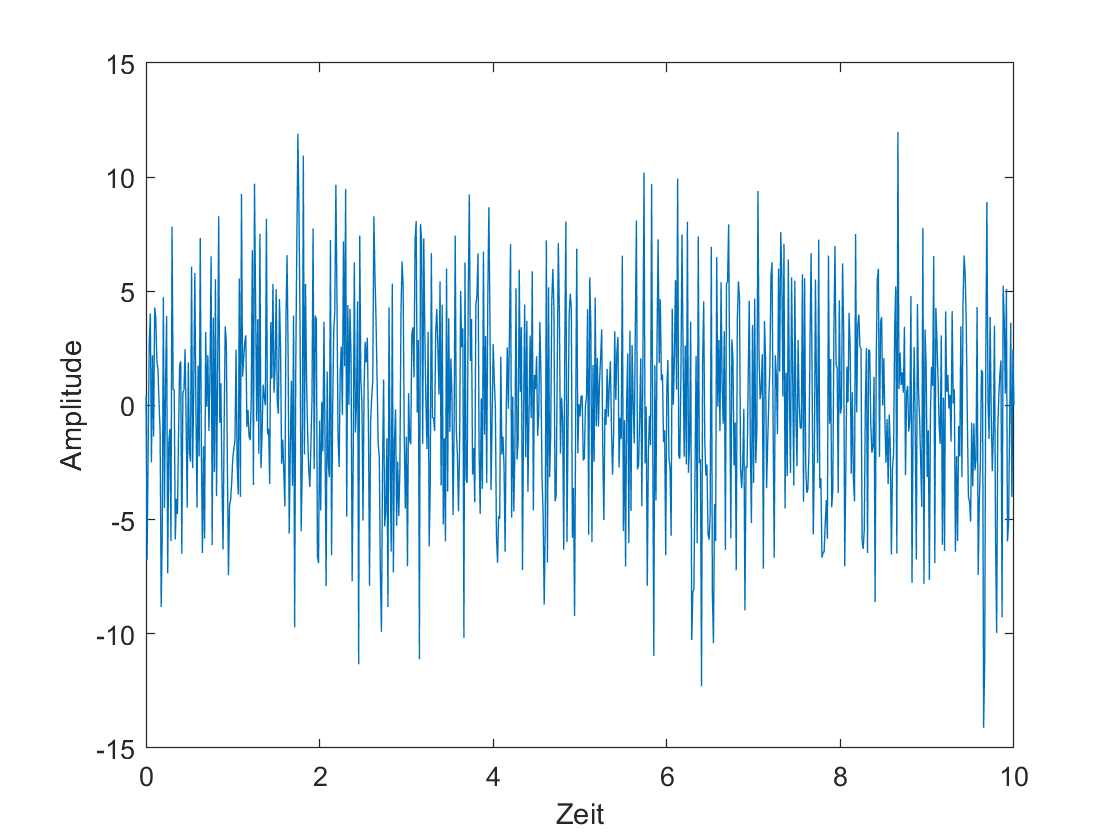
\includegraphics[width=\linewidth]{papers/brown/images/weissesRauschen.png}
		\caption{Echtes weisses Rauschen}
		\label{weissesRauschenSignal}
	\end{minipage}
	\hspace{0.05\linewidth}
	\begin{minipage}{0.45\textwidth}
		\centering
		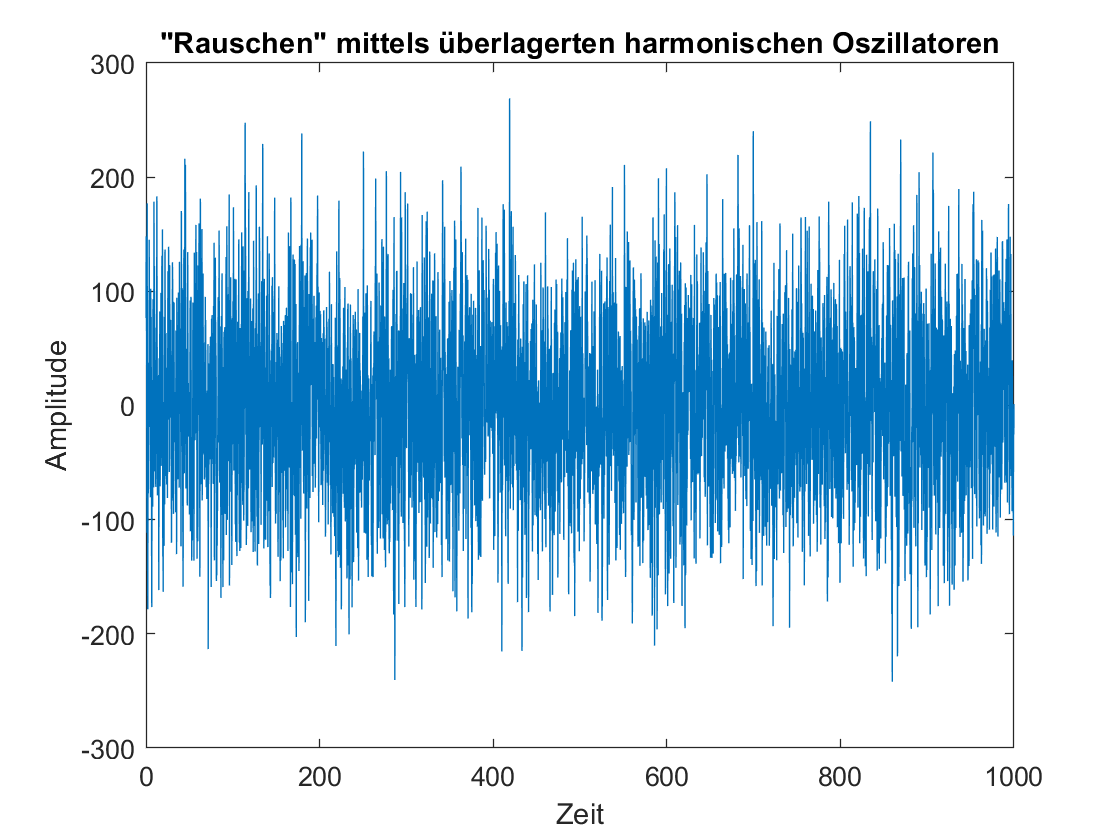
\includegraphics[width=\linewidth]{papers/brown/images/RauschenDurchUeberlagerteHarmonsicheSchwingungen.png}
		\caption{Überlagerte harmonische Schwingungen}
		\label{überlagerteSchwingungen}
	\end{minipage}
	\begin{minipage}{0.45\textwidth}
		\centering
		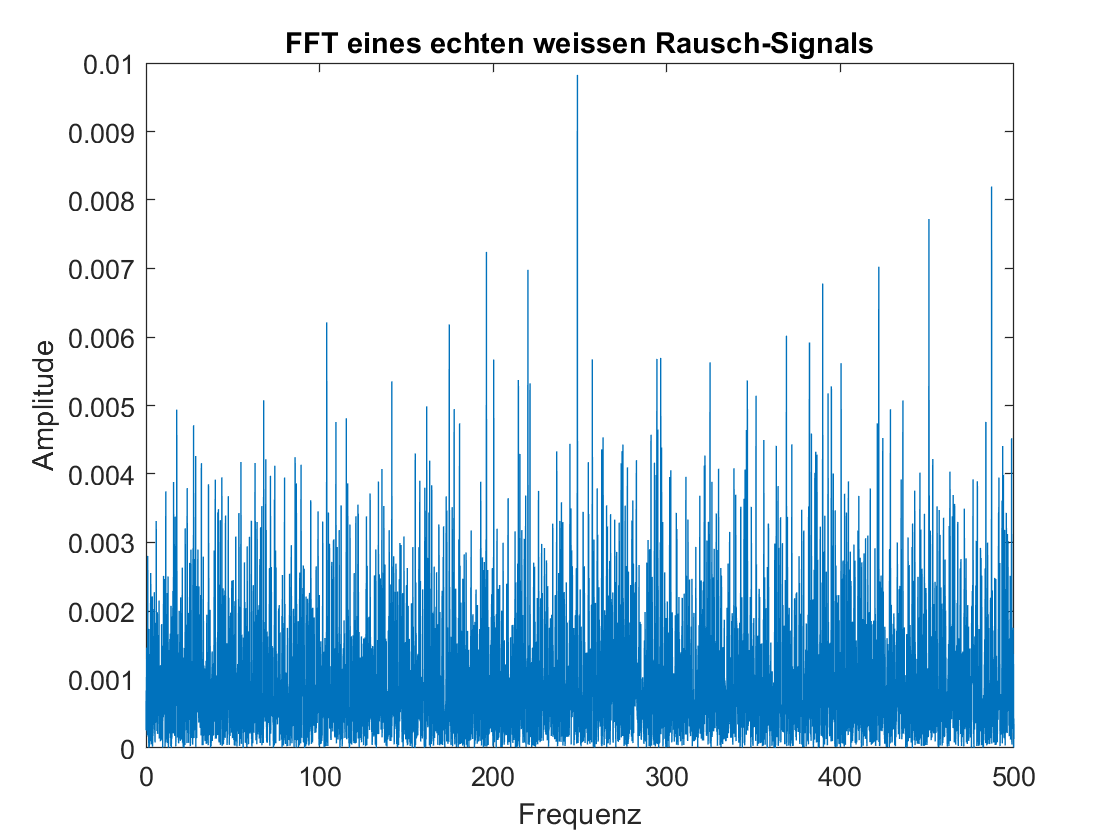
\includegraphics[width=\linewidth]{papers/brown/images/FFTweissesRauschen.png}
		\caption{FFT eines weissen Rausch-Signals}
		\label{FFTweissesRauschen}
	\end{minipage}
	\hspace{0.05\linewidth}
	\begin{minipage}{0.45\textwidth}
		\centering
		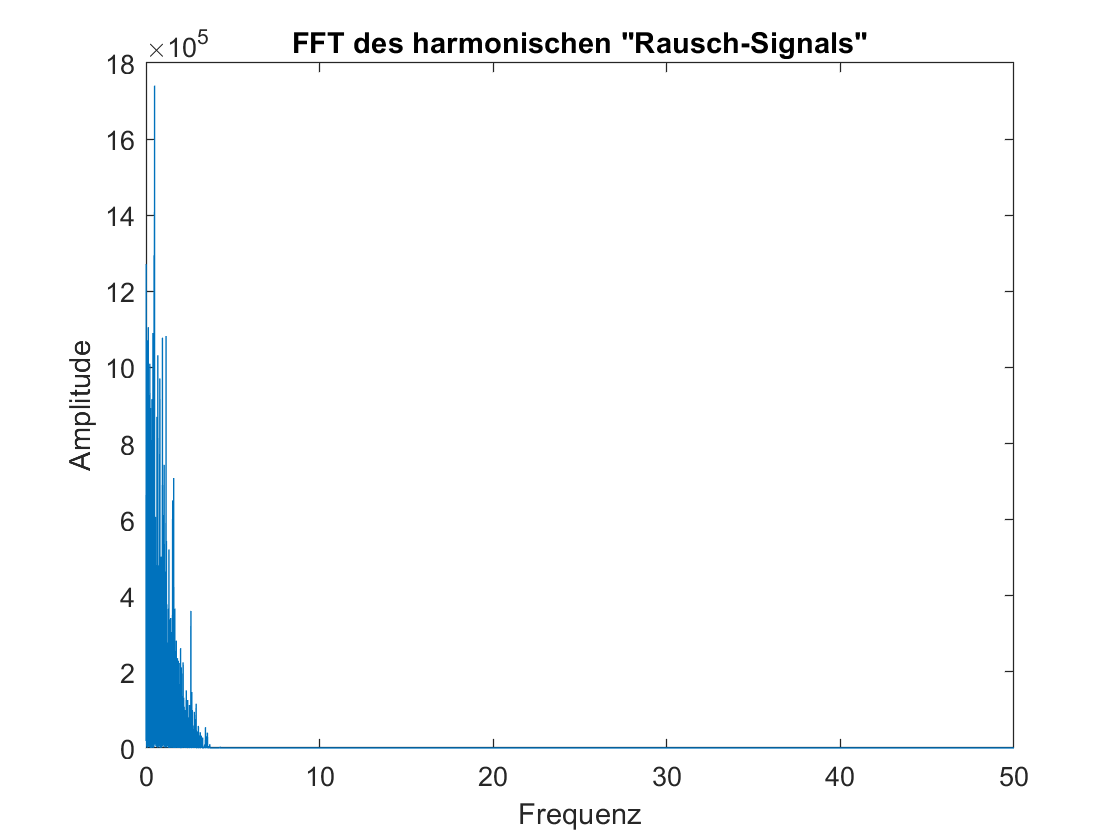
\includegraphics[width=\linewidth]{papers/brown/images/FFT-ueberlagerteSchwingungen.png}
		\caption{FFT von überlagerten harmonischen Schwingungen}
		\label{FFTüberlagerteSchwingungen}
	\end{minipage}
\end{figure}


\subsection{Rauschen mittels Random Walk oder Wiener Prozess\label{brown:Rauschen:RandomWalkWiener}}

Um Rauschen zu modellieren muss als Grundlage ein stochastischer Prozess definiert werden. Zwei weit verbreitete Konzepte sind dabei der \textit{random walk} und der Wienerprozess.

\begin{definition}\textbf{Random Walk:}
	\label{randomWalk}
	Bei einem Random Walk beginnt man an einem Ausgangspunkt (normalerweise 0) und macht bei jedem Zeitschritt eine zufällige Schritt vor oder zurück. Oft dient dazu die Binominalverteilung, wobei auch asymmetrische Verteilungen verwendet werden können. Die Schrittlänge und Richtung kann ebenfalls durch eine unabhängige Wahrscheinlichkeitsverteilung bestimmt werden order als konstant definiert werden. Dieses Verfahren zeichnet sich durch eine einfache numerische Implementation aus, da es per Definition schon diskret ist.
\end{definition}

\begin{definition}\textbf{Wiener-Prozess:}
	\label{wienerprozess}
	Der Wiener-Prozess ist ein kontinuierlicher stochastischer Prozess. Er kann als Grenzwert eines Random Walks erachtet werden, sofern die Zeitschritte gegen null gehen und die Schrittlängen normalverteilt sind. Speziell dabei ist, dass unabhängig von der verstrichenen Zeit der Erwartungswert dem Ausgangswert entspricht.
\end{definition}

Der Wienerprozess muss also folgende Eigenschaften erfüllen: 

%Man könnte also den Random Walk als eine diskrete Version eines Wiener-Prozesses bezeichnen oder umgekehrt, dass ein Wiener-Prozess eine kontinuierliche Version eines Random Walks ist. Sie unterscheiden sich jedoch bezüglich ihrer zeitlichen Diskretisierung und in den verwendeten Wahrscheinlichkeitsverteilungen.


\begin{enumerate}
	\item $ W(0) = 0 $; Der Startwert von $ t = 0 $ ist 0.
	\item $ W(t_{1}) - W(t_{2}) $ ist ein normalverteilte Zufalls-Variable mit Erwartungswert 0 und Varianz $ t_{1} - t_{2} $.
	\item Zu jedem weiteren Zeitpunkt $ t_{n} $ ist die Zufalls-Variable unabhängig von allen vorhergehenden Werten. Dies wird auch die Markow-Eigenschaft genannt, wenn der Übergang in einen neuen Zustand nicht vom vorherigen Verlauf abhängt.
\end{enumerate}

Weiter wird auf den Wienerprozess jedoch nicht eingegangen, da dieser ausführlich im Kapitel \glqq \textit{8.1 Modell für Rauschen: der Wiener-Prozess}\glqq{} des Buches vom Mathematischen Seminar über Differenzialgleichungen beschrieben wird.


\subsection{Implikationen\label{brown:Rauschen:Implikationen}}

Eines der grössten Probleme im Zusammenhang mit Rauschen ist die Differenzierbarkeit. Dies ist häufig beim Umgang mit Mess-Signalen Fall. Die eigentliche Messung ist gestört, was das bestimmen einer lokalen Steigung und somit die Äderungsrate der Messgrösse verfälschen kann. Auch empfangene daten-Signale sind oft verrauscht, was das Dekodieren der darin enthaltenen Information erschwert oder sogar verfälscht.

Die einfachste Methode und häufig auch ein erster Schritt in der Signalverarbeitung, ist die Anwendung eines Tiefpass- oder Bandpass-Filters. Dieser entfernt jedoch nicht nur das Rauschen, sondern auch ein Teil der im Signal enthaltenen Information.

\begin{figure}
	\centering
	\begin{minipage}{0.45\textwidth}
		\centering
		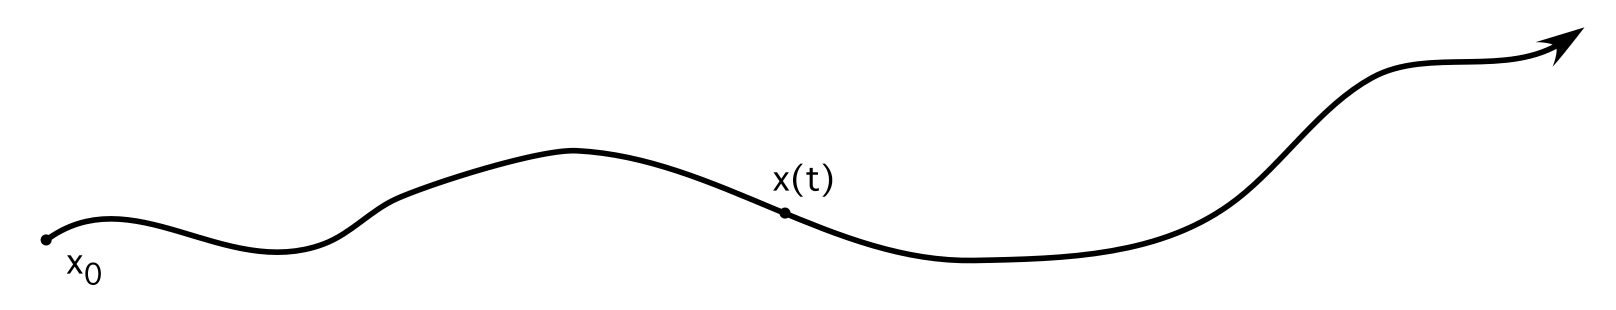
\includegraphics[width=0.9\textwidth]{papers/brown/images/idealSignal.png}
		\caption{Ideales Signal}
		\label{idealSignal}
	\end{minipage}
	\hspace{0.05\linewidth}
	\begin{minipage}{0.45\textwidth}
		\centering
		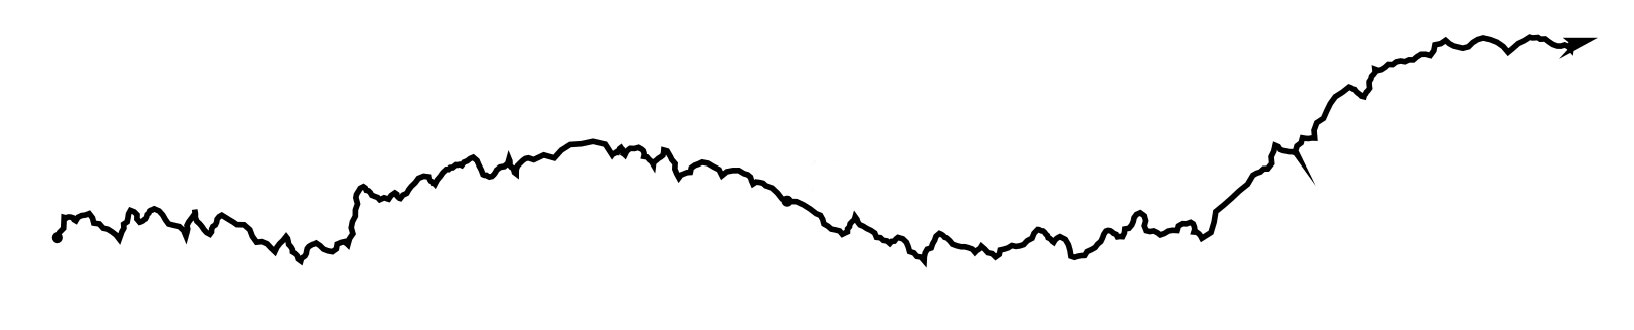
\includegraphics[width=0.9\textwidth]{papers/brown/images/realSignal.png}
		\caption{Reales Signal}
		\label{realSignal}
	\end{minipage}
\end{figure}

Eine weitere Schwierigkeit entsteht, wenn anhand von Messdaten ein Modell erstellt werden soll, welches das Verhalten der Messdaten widerspiegelt. Dabei kann es sein, dass man das Rauschen als Teil des Systems sieht oder rein als externe Störung. Im einen Fall muss zwischen System und Rauschen unterschieden werden, im anderen Fall muss das System Rauschen abbilden können.
%mehr dazu schreiben?
% Absatz?

Ist ein System anhand einer gewöhnlichen Differenzialgleichung (DGL) gegeben, kann das Verhalten des Systems unter Berücksichtigung der Anfangsbedingungen vorhergesagt werden. Vom Anfangswert aus entwickelt sich die Funktion gemäss der Startbedingung und dem durch die DGL gegebenen Vektorfeld. 

In vielen Bereichen entspricht ein solch deterministisches System  nicht der Realität und suggeriert eine Aussagekraft, welche sich nicht mit Beobachtungen deckt. Es gibt viele Systemen, welche stark auf kleine Störeinflüsse reagieren. Dies führt dazu, dass sich die Lösung einer DGL gegenüber der Realität, zum Beispiel durch Rauschen, nicht perfekt deckt oder das Resultat sogar komplett divergiert. .

Ein gutes Beispiel dafür ist folgendes System:
\begin{equation}
	\frac{dx}{dt} = - y 
\end{equation}
	
\begin{equation}
	\frac{dy}{dt} = x^2 + y
	\label{divergentEquation}
\end{equation}

In der Abbildung~\ref{divergentAndConvergentSystem} sind zwei unterschiedliche Trajektorien im Vektorfeld eingezeichnet, welches durch die Gleichung~\ref{divergentEquation} gegeben ist. In rot ist der Verlauf im Intervall  $ t = [0, 3] $ mit dem Startwert $ (-1.7, -1.4) $ gegeben und in grün mit dem Startwert $ (-1.8, -1.4) $.

\begin{figure}
	\centering
	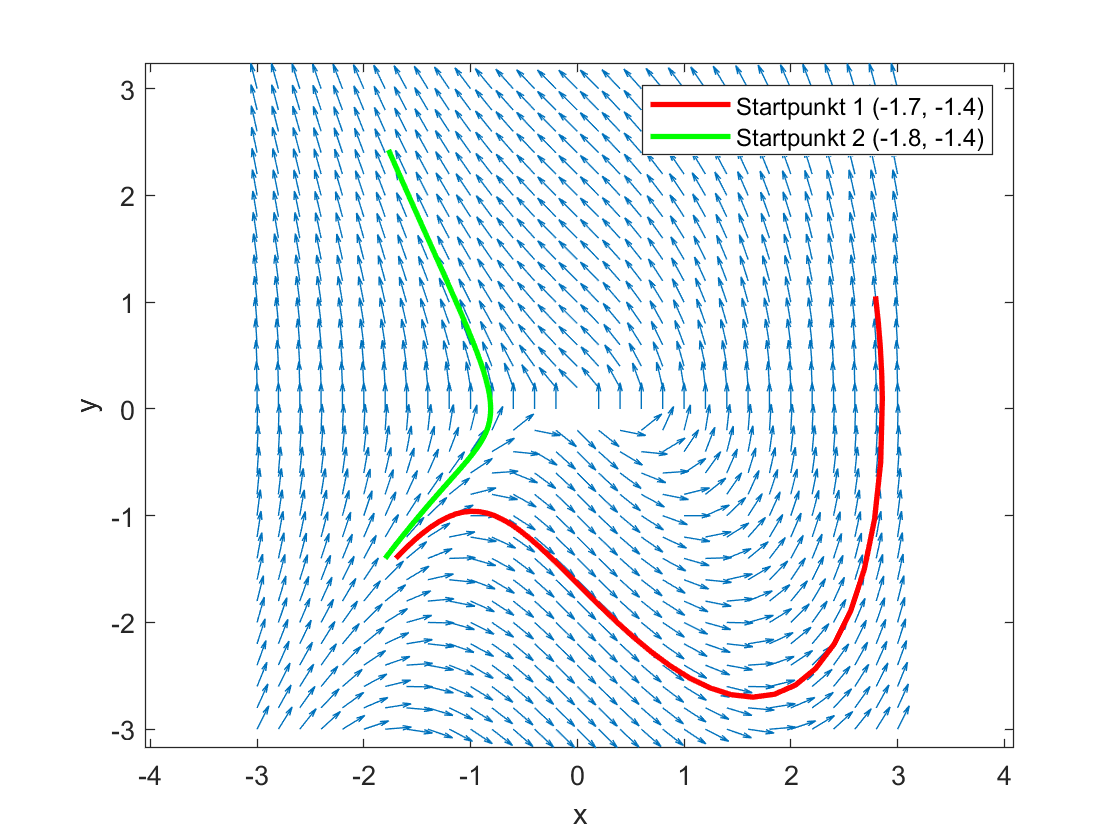
\includegraphics[width=0.8\textwidth]{papers/brown/images/Vektorfeld-mit-zwei-Pfaden.png}
	\caption{Zwei Pfade mit fast gleichem Startpunkt}
	\label{divergentAndConvergentSystem}
\end{figure}

Dieses System veranschaulicht schön, wie sich eine kleine Störung der Startbedingung auf den Verlauf der Lösung auswirken kann. In diesem speziellen Fall konvergieren die Lösung zu einem späteren Zeitpunkt $ t $ wieder. Bedenkt man nun, dass eine solche Störung durch Rauschen herbeigeführt werden könnte, scheint es unsinnig eine einzige fixe Lösung für ein solches System anzugeben - zumindest nicht ohne auf die Aussagekraft der Lösung unter Rauscheinfluss hinzuweisen oder den Lösungsraum genauer zu spezifizieren.


Es gibt auch Systeme, welche bei kleinen Störungen aus einem stabilen Zustand in einen instabilen Zustand übergehen und komplett divergieren. In solchen Fällen kann es ein fataler Fehler sein, zufällige Störungen des Systems nicht zu berücksichtigen. Andere Systeme beinhalten selbst eine zufällige Komponente, welche nicht vernachlässigt werden soll.

Um diesem Umstand gerecht zu werden, kann man die Möglichkeit von zufälligen Störungen beim Aufstellen eines Modells miteinbeziehen (in diesem Fall \textit{white noise}). Anstatt eine fixe Lösung zum Zeitpunkt $ t $ anzugeben, kann man eine Wahrscheinlichkeitsverteilung über die verschiedenen möglichen Endzustände angeben - et. voilà, man hat den Lösungsraum einer stochastische Differenzialgleichung (SDGL).
